%\documentclass[10pt, handout]{beamer}
\documentclass[10pt, presentation]{beamer}

\usefonttheme{professionalfonts}

\usepackage{amsmath, amsfonts, amssymb, amsthm}
\usepackage[numbers,sort&compress]{natbib}
\usepackage{graphicx}
\usepackage{graphics}
\usepackage{multirow}
\usepackage{color}
\usepackage{url}
\usepackage{hyperref}

\usepackage[plain,noend]{algorithm2e}
\usepackage{setspace}
\usepackage{bm}

\usepackage{pifont}
\usepackage{eurosym}
\usepackage{palatino}
\usepackage{multimedia}
\usepackage{wasysym}
\usepackage{fancybox}
\usepackage{mathrsfs}
\usepackage{subfigure}
\usepackage{wrapfig}

\usepackage{units}
\usepackage{ifthen}
\usepackage{tikz}
\usetikzlibrary{fit,positioning,arrows,automata}

\usepackage{Teaching}

\usetheme{metropolis}
\metroset{block=fill}
\setbeamertemplate{frame numbering}[fraction]

% Title page
\title{Statistical Methods for Population Health}
\subtitle{Week 1: Introduction to Statistics}

\author{Ruoqing Zhu, Ph.D. \href{mailto:rqzhu@illinois.edu}{\footnotesize $<$rqzhu@illinois.edu$>$}}
\institute{Department of Statistics \\ University Illinois Urbana-Champaign}

\date{\scriptsize \today}

\begin{document}

\frame{\titlepage}

\frame{
\frametitle{Welcome!}
    \begin{itemize}
        \item Welcome to the Statistics section!
        \item<2-> This is a sequence of three lectures (I call them guided TBL)
        \item<3-> \alert{Core skills}
        \begin{itemize}
            \item Statistical principles
            \item Result interpretation
            \item Basic data analysis using R
            \item Some modeling techniques
        \end{itemize}
    \end{itemize}
}

\frame{
\frametitle{Weekly Schedule}
    \begin{itemize}
        \item<1-7> Week 1: R Introduction and Statistical Principles
        \item<3-6> Week 2: Testing Mean Differences and Associations
        \item<4-6> Week 3: Statistical Models for Multivariate Analysis
    \end{itemize}
}

\section{The Lady Tasting Tea}

\frame{
\frametitle{The Lady Tasting Tea Problem}
\begin{columns}[c]
\column{2.5in}
\begin{itemize}
\item In 1920s Cambridge, England, a Lady, named Muriel Bristol, claimed to be able to tell \alert{whether the tea or the milk was added first} by the taste of it!
\uncover<2->{ \item A statistician Ronald Fisher what to test if thats true or not using \alert{probability principles}}
\end{itemize}
\column{1.5in}
\uncover<1->{
\begin{figure}
    \centering
    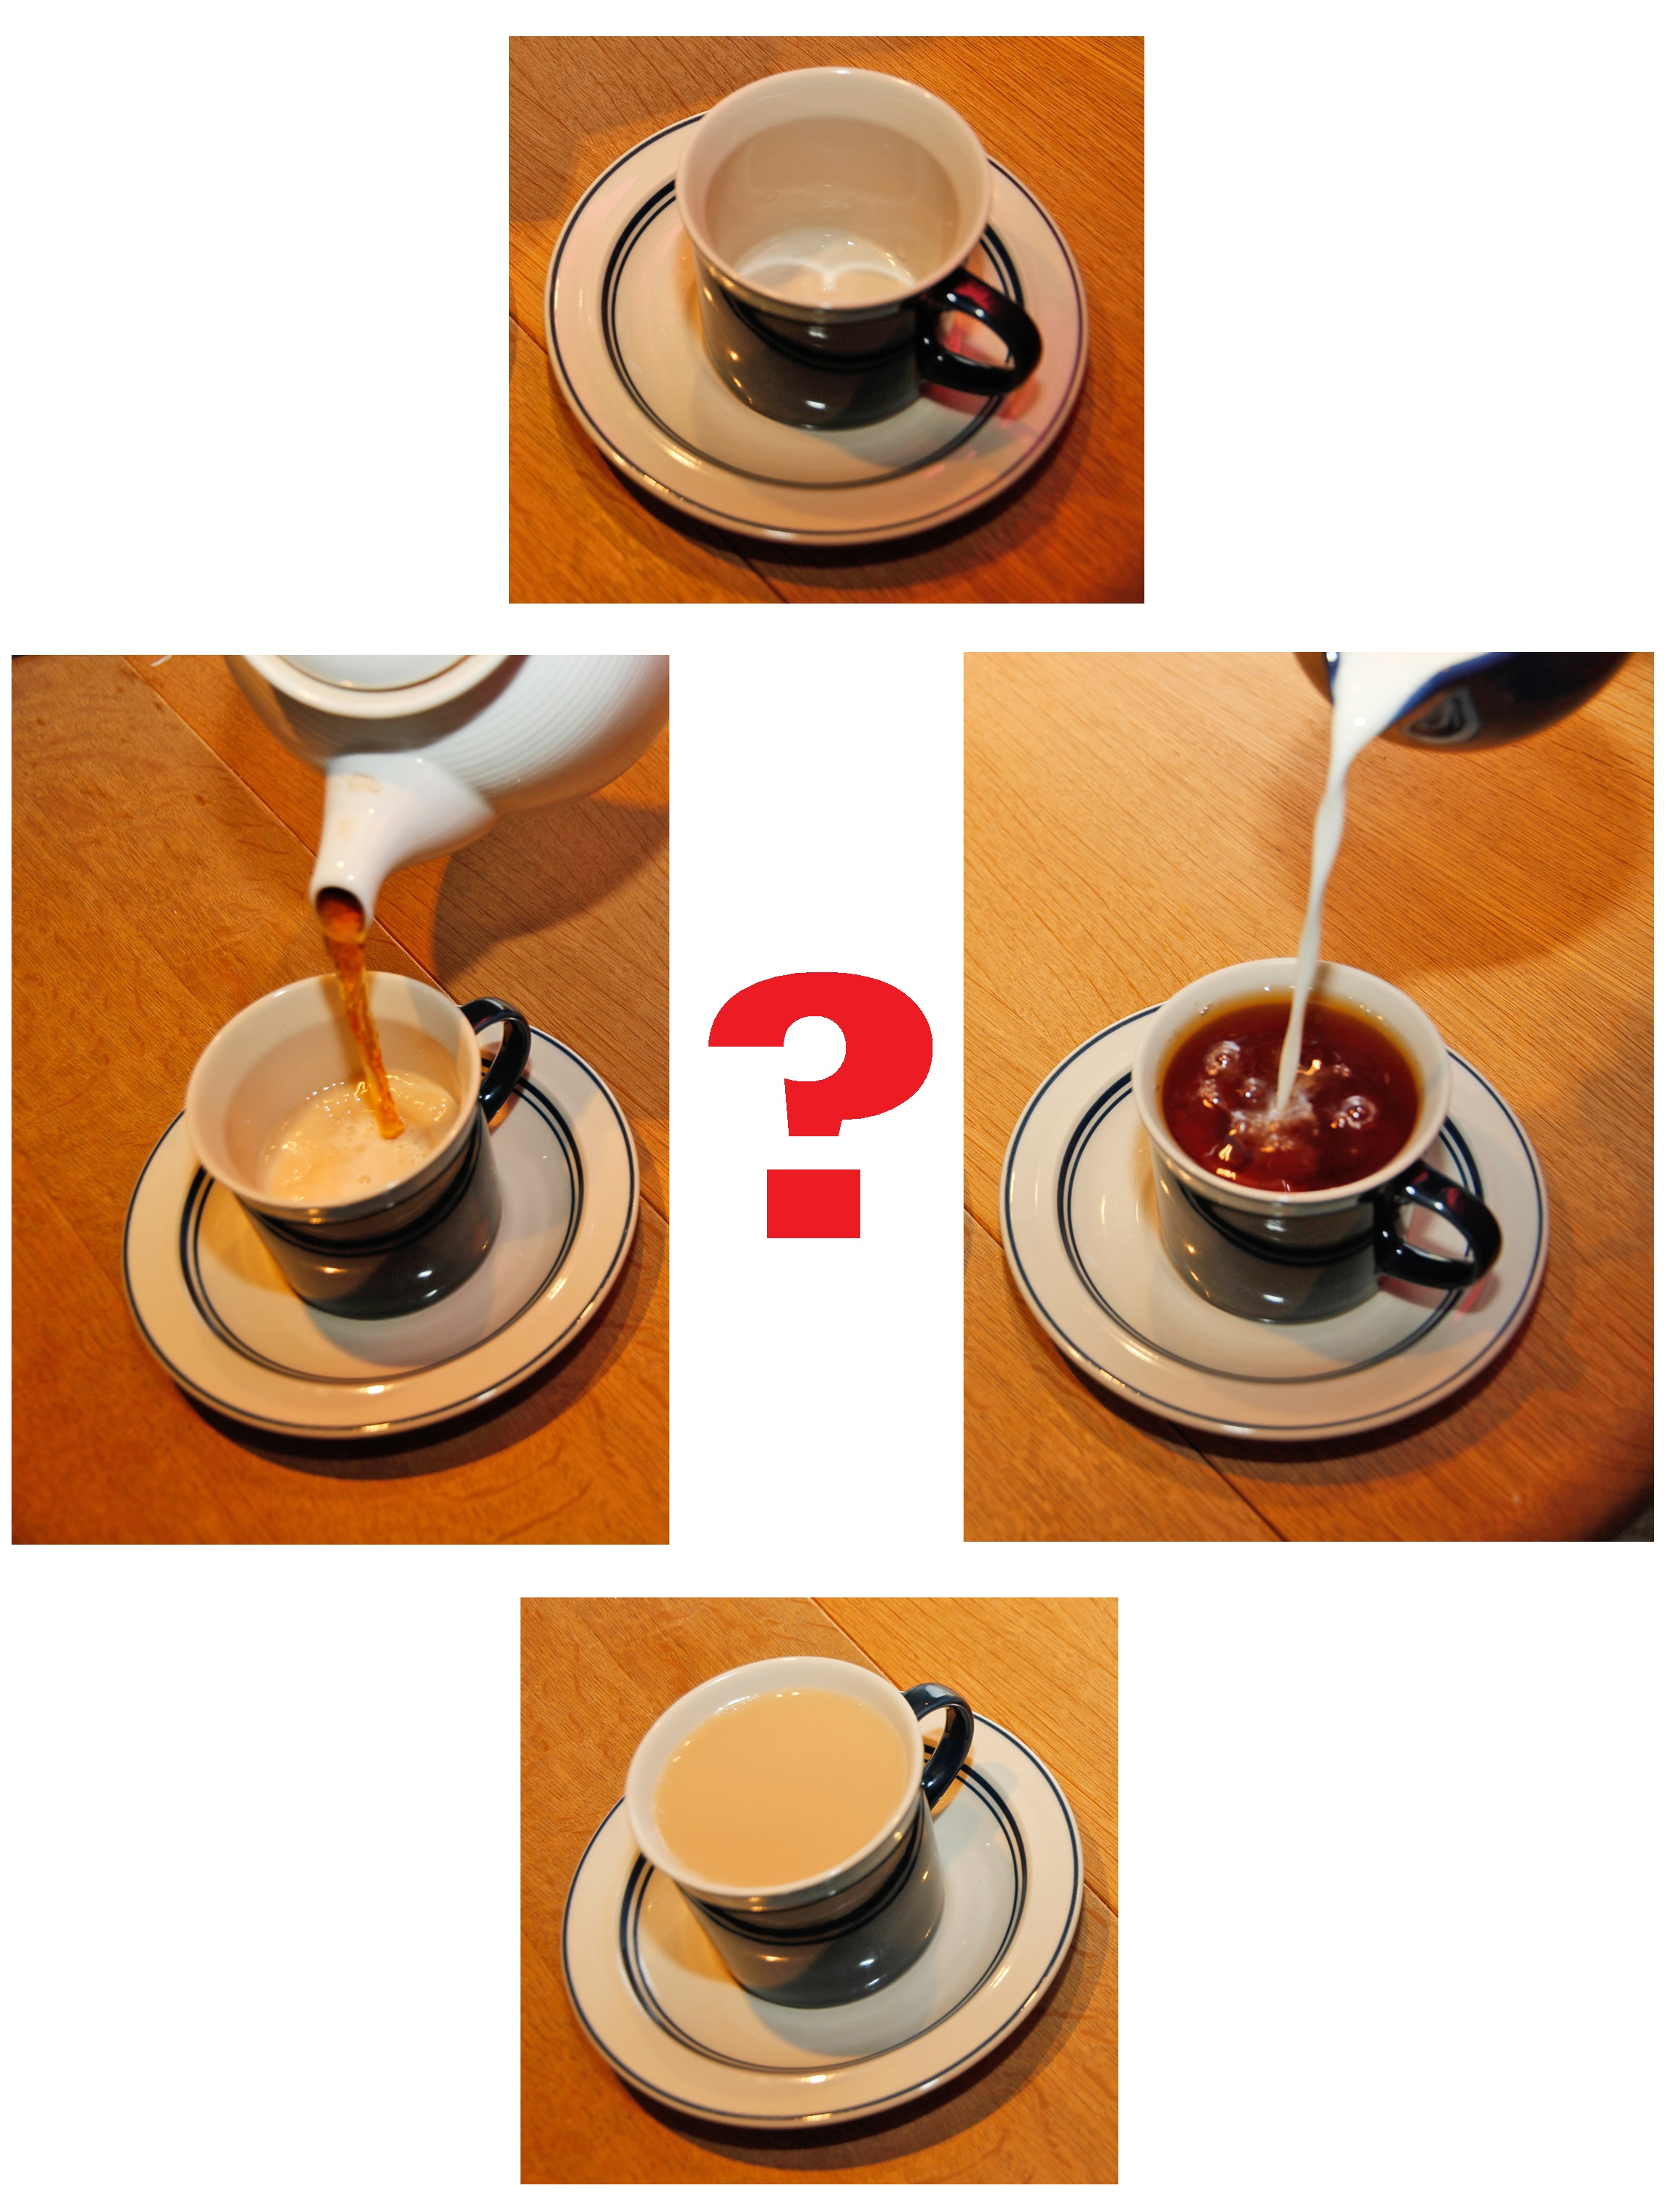
\includegraphics[scale=0.05]{plots//Tea_Milk2.jpg}
\end{figure}
}
\end{columns}
\tiny ``The Lady Tasting Tea: How Statistics Revolutionized Science in the Twentieth Century'' (2001) by David Salsburg
}


\frame{
\frametitle{The Essential Idea}
\begin{itemize}
    \item Suppose Lady Bristol \alert{does not have that ability}, then she will be \alert{randomly guessing}
    \item<2-> Let's \alert{prepare many cups of tea} for her to identify, then we would expect her to identify, \alert{on average, half} of them correctly.
    \item<3-> However, if she can identify \alert{many} of them correctly, then we may have to \alert{reject the assumption of random guessing}
    \item<4-> The question is, \alert{how many is too many?}
\end{itemize}
}


\frame{
\frametitle{The Essential Idea}
\begin{columns}[c]
\column{1.8in}
\begin{itemize}
    \item Two important concepts:
    \begin{itemize}
    \item[1.] Experimental design
    \item[2.] Hypothesis testing
    \end{itemize}
\end{itemize}
\column{1.5in}
\begin{figure}
    \centering
    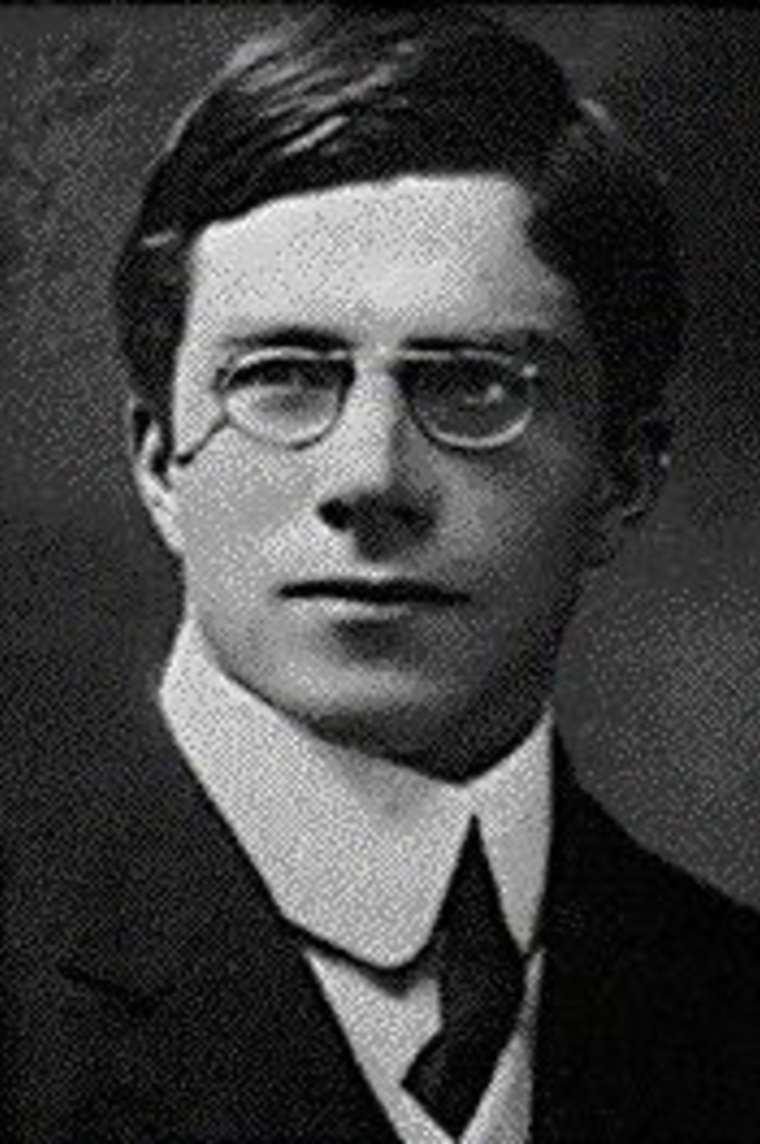
\includegraphics[scale=0.2]{plots//Fisher.jpg}\\
    Sir Ronald A. Fisher\\
    (1890 - 1962)
\end{figure}
\end{columns}
}

\frame{
\frametitle{Fisher's Exact Test}
\begin{itemize}
    \item<1-> Fisher prepared 8 cups of tea, 4 with milk added first and 4 with tea added first.
    \item<2-> Lady Bristol was asked to identify them
    \item<2-> There are totally $\frac{8!}{4!(8-4)!} = 70$ possible results. \alert{If she is randomly guessing}, then each result has equal chance:
    \begin{itemize}
        \item<3-> The chance of identifying all 4 correctly is 1/70
        \item<3-> The chance of 3 is 16/70
        \item<3-> The chance of 2 is 36/70
        \item<3-> The chance of 1 is 16/70
        \item<3-> The chance of 0 is 1/70
    \end{itemize}
    \item<4-> What can be considered as \alert{``surprising'' evidence} given the assumption that she is randomly guessing?
\end{itemize}
}

\frame{
\frametitle{Fisher's Exact Test}
    \begin{itemize}
        \item Fisher used \alert{0.05} as the cut-off:\\
        $\qquad$ \alert{If the actual result falls into the top 5\% of the most extreme cases, we consider this as a surprising evidence and claim that she is not randomly guessing.}
        \item<2-> How many cups Lady Bristol identified correctly?
    \end{itemize}
}

\frame{
\frametitle{Recap}
Some \underline{\textbf{key steps}} in hypothesis testing:
\begin{itemize}
    \item[1).] Form \alert{Null and Alternative} hypotheses:
    $$ \alert{\text{Null $H_0$}}: \text{Random Guessing} \quad \text{vs.} \quad \alert{\text{Alt. $H_1$}}: \text{Not Random Guessing}$$
    \item[2).]<2-> Perform an experiment and \alert{observe} that the lady identified the 4 correctly.
    \item[3).]<3-> \alert{If the Null hypothesis is correct}, there is only 1.4\% chance that one can guess 4 correctly
    \item[4).]<4-> This is a ``small probability event'' (smaller than a pre-determined \alert{significance level}, $\alpha = 0.05$), so we will make a conclusion to \alert{reject the Null}.
\end{itemize}
}

\frame{
\frametitle{Recap}
\begin{itemize}
    \item If we reject the Null hypothesis, does it mean that Lady Bristol actually has the ability to identify them?
\end{itemize}
}

\frame{
\frametitle{Correct or Wrong decision?}
\begin{itemize}
    \item We could still make a wrong decision. In fact, there are four situations:
    \vspace{0.5cm}
    \begin{center}
    \begin{tabular}{|c|cc|}
    \hline
     & Accept $H_0$ & Reject $H_0$\\
    \hline
    $H_0$ true & $\checkmark$ & \alert{Type I Error} \\
    $H_0$ false & \alert{Type II Error} & $\checkmark$ \\
    \hline
    \end{tabular}
    \end{center}
    \vspace{0.5cm}
    \item \alert{Type I error}: $H_0$ true but we reject it.
    \item \alert{Type II error}: $H_0$ false but we accept it.
\end{itemize}
}


\frame{
\frametitle{Correct or Wrong decision?}
\begin{itemize}
    \item \alert{Type I error} can be controlled using the $\alpha$ level we choose.
    \item \alert{1 $-$ Type I error} is called the confidence level
    \item<2-> \alert{Type II error} is difficult to analyze because we don't know what the alternative may look like. For example, the lady may have 0.7 probability to identify a correct one, or 0.9, 0.51, etc. They all can have different Type II errors.
    \item<2-> \alert{1 $-$ Type II error} is called the power.
\end{itemize}
}


\frame{
\frametitle{Summary}
\begin{itemize}
    \item Statistics is a tool to analyze data and find patterns
    \item However, statistics cannot provide a definitive answer
    \item Definitive answers come from understanding the science
\end{itemize}
}

\frame{
\frametitle{Homework}
    \begin{itemize}
        \item Further reading (textbook): Sections 11.3.3 and 11.3.4
        \begin{itemize}
            \item ``\alert{Quantitative methods for health research: a practical interactive guide to epidemiology and statistics}'' by Nigel Bruce, Daniel Pope, Debbi Stanistreet. Hoboken, NJ:Wiley, 2018 2nd edition. Wiley Online Library [\href{https://scholar.google.com/scholar?hl=en\&as_sdt=0\%2C14\&q=Quantitative+methods+for+health+research\%3A+a+practical+interactive+guide+to+epidemiology+and+statistics\&btnG=}{Download Link}]
        \end{itemize}
        \item Install \href{https://www.rstudio.com/products/rstudio/download/\#download}{RStudio} and \href{https://www.r-project.org/}{R}
    \end{itemize}
}


\end{document}
